%% 
%% Copyright 2007, 2008, 2009 Elsevier Ltd
%% 
%% This file is part of the 'Elsarticle Bundle'.
%% ---------------------------------------------
%% 
%% It may be distributed under the conditions of the LaTeX Project Public
%% License, either version 1.2 of this license or (at your option) any
%% later version.  The latest version of this license is in
%%    http://www.latex-project.org/lppl.txt
%% and version 1.2 or later is part of all distributions of LaTeX
%% version 1999/12/01 or later.
%% 
%% The list of all files belonging to the 'Elsarticle Bundle' is
%% given in the file `manifest.txt'.
%% 
%% Template article for Elsevier's document class `elsarticle'
%% with harvard style bibliographic references
%% SP 2008/03/01

%\documentclass[preprint,12pt,authoryear]{elsarticle}  %default in the template
%\documentclass[preprint,10pt,authoryear]{elsarticle}

%% Use the option review to obtain double line spacing
%% \documentclass[authoryear,preprint,review,12pt]{elsarticle}

%% Use the options 1p,twocolumn; 3p; 3p,twocolumn; 5p; or 5p,twocolumn
%% for a journal layout:
%% \documentclass[final,1p,times,authoryear]{elsarticle}
%% \documentclass[final,1p,times,twocolumn,authoryear]{elsarticle}
 \documentclass[final,3p,times,authoryear]{elsarticle}
%% \documentclass[final,3p,times,twocolumn,authoryear]{elsarticle}
%% \documentclass[final,5p,times,authoryear]{elsarticle}
%% \documentclass[final,5p,times,twocolumn,authoryear]{elsarticle}

%% For including figures, graphicx.sty has been loaded in
%% elsarticle.cls. If you prefer to use the old commands
%% please give \usepackage{epsfig}

%% The amssymb package provides various useful mathematical symbols
\usepackage{amssymb}
%% The amsthm package provides extended theorem environments
 \usepackage{amsthm}
 \usepackage{amsmath}
 \usepackage{color}
 \usepackage{amsmath}
\usepackage{siunitx}


\usepackage{framed} % Framing content
\usepackage{multicol} % Multiple columns environment
\usepackage{nomencl} % Nomenclature package
\makenomenclature
%\setlength{\nomitemsep}{-\parskip} % Baseline skip between items
\setlength{\nomitemsep}{0.01cm}
\renewcommand*\nompreamble{\begin{multicols}{2}}
\renewcommand*\nompostamble{\end{multicols}}
\newcommand{\degreeC}{\ensuremath{^\circ}C }

\usepackage{eurosym}

\usepackage[nonumberlist]{glossaries}
\makeglossaries 


%% The lineno packages adds line numbers. Start line numbering with
%% \begin{linenumbers}, end it with \end{linenumbers}. Or switch it on
%% for the whole article with \linenumbers.
%% \usepackage{lineno}

\journal{Urban Climate}

\newglossaryentry{aa}{name={$a$},symbol={\ensuremath{a}},description={a}}

\begin{document}

\begin{frontmatter}

%% Title, authors and addresses

%% use the tnoteref command within \title for footnotes;
%% use the tnotetext command for theassociated footnote;
%% use the fnref command within \author or \address for footnotes;
%% use the fntext command for theassociated footnote;
%% use the corref command within \author for corresponding author footnotes;
%% use the cortext command for theassociated footnote;
%% use the ead command for the email address,
%% and the form \ead[url] for the home page:
%% \title{Title\tnoteref{label1}}
%% \tnotetext[label1]{}
%% \author{Name\corref{cor1}\fnref{label2}}
%% \ead{email address}
%% \ead[url]{home page}
%% \fntext[label2]{}
%% \cortext[cor1]{}
%% \address{Address\fnref{label3}}
%% \fntext[label3]{}

\title{The Paris end of town? Urban typology through machine learning.} 




%% use optional labels to link authors explicitly to addresses:
\author[melb,monash]{Kerry A. Nice}
\corref{cor1}
\ead{kerry.nice@unimelb.edu.au}
\cortext[cor1]{Principal corresponding author}

\author[melb]{Jason Thompson} 
\author[melb]{Jasper Wijnands} 
\author[melb]{Gideon Aschwanden} 
\author[melb]{Mark Stevenson} 

\address[melb]{Transport, Health, and Urban Design Hub, Faculty of Architecture, Building, and Planning, University of Melbourne, Victoria 3010, Australia}
\address[monash]{School of Earth, Atmosphere and Environment, Monash University, Clayton, Australia}
\begin{abstract}

The confluence of recent advances in availability of geospatial information, computing power, and artificial intelligence offers new opportunities to understand how and where our cities differ and also, how they are alike. Departing from a traditional `top-down' analysis of urban design features, this project analyses thousands of images of urban form (consisting of street view and satellite imagery as well as street maps) from each Australian state and territory capital city, before making comparisons to a group of 20 other high profile cities from around the world including London, Paris, Copenhagen, Beijing, Los Angeles, and New York. We then map these international cities across each Australian example to produce within-city locations that demonstrate the closest connections between these areas and their international comparators. Finally, we suggest relationships between urban design and consequent transport, environmental, and population health outcomes these comparisons suggest may be generated by each location. This work demonstrates an entirely new and highly efficient method for understanding the relationship between cities around the world, and the health, transport, and environmental consequences of their design. Perhaps most importantly, it also answers the age-old question, ``Is there really a `Paris-end' of your city?''.



%\nomenclature{$T_{mrt}$}{mean radiant temperature (\SI{}{\degreeCelsius})}  
%\nomenclature{$UTCI$}{universal thermal climate index}
\end{abstract}

\begin{keyword}
machine learning, urban typology, urban design, transport and health

%% PACS codes here, in the form: \PACS code \sep code

%% MSC codes here, in the form: \MSC code \sep code
%% or \MSC[2008] code \sep code (2000 is the default)

\end{keyword}

\end{frontmatter}

%\begin{table*}[!t]   
%\begin{framed}
%\printnomenclature
%%\input{VTUF-3DDesign_Nomenclature}
%\end{framed}
%\end{table*}



%% \linenumbers

%% main text




\section{Introduction}\label{sec:introduction}



 
In 2013, 65\% of Australians lived in capital cities and it is estimated that this will increase to 72\% by 2053  \citep{ABS2008}. These projections are reflected in population growth estimates that will see the country’s population likely increase from 24 million today to over 33 million by 2050  \citep{ABS2008}. This growth is expected to mostly take place within the four largest capital cities (Sydney, Melbourne, Brisbane and Perth) with projections indicating that by 2053 both Sydney and Melbourne will have populations of almost 8 million  \citep{CommonwealthofAustralia2010}. As a consequence of this population growth, an array of transportation and population health challenges will emerge.

The importance of integrating transport plans with decisions regarding land-use is being recognised by governments \citep{ATAP2016,SA2015}. Land-use decisions significantly influence transport options and travel choice. Further, the high levels of low-density suburbanisation and high car dependency that characterise many Australian and New Zealand cities are remnants of a mid-twentieth century focus on home and car ownership \citep{Currie2007,Dodson2008}. As a consequence, the status and practical utility of cycling or walking for daily travel requirements is limited \citep{Heesch2014,Daley2011}. Low-density housing renders the cost of large-scale public transport prohibitive, producing a reliance on private vehicles and increasing exposure to risks associated with traffic speed, volume, emissions, and physical inactivity  \citep{Cepeda2016,MingWen2008,Norman2006}. Although some progress has been made in promoting active modes of transport the percentage of Australians walking or cycling to work remains low and primarily concentrated in low-speed, inner-city areas where distances are minimal. Public health policy-makers and urban/transport planners have an opportunity to change this situation by embracing strategies that proactively support active transport modes as facilitated by urban designs witnessed in other countries around the world.

For example, Copenhagen's significant long-term investment in cycling infrastructure of over \euro 30 million in cycling infrastructure for a city of approximately 550,000 residents has seen its rates of cycling mode share expand to 45\% of all trips without consequent increases in road trauma \citep{Kaplan2014}. Similarly, Amsterdam's (and the Netherlands more generally) continued leadership in active transport promotion has demonstrated that cycling and walking can be re-claimed in areas and streets previously lost to car traffic, producing both health and economic benefit \citep{Andersen2000}. Substantial published evidence indicates that land-use affects transport modal choice and behaviour  \citep{Giles-corti2016,Kleinert2016,Goenka2016}. In addition, improved population health outcomes related to chronic conditions such as respiratory disease, cardiovascular disease, and Type 2 diabetes are strongly linked with more active transport modal choices  \citep{Zapata-Diomedi2017}. Therefore, the creation of cities and precincts that facilitate greater uptake of safe, active transport could produce manifold environmental, productivity, and population health benefits. 

However, understanding the association between urban design features and health or environmental outcomes remains difficult, especially when underlying data, locations, methods, and demographics upon which statistical models are built vary considerably across studies. The confluence of recent advances in availability of geospatial information, computing power, and artificial intelligence offers new opportunities to understand how and where our cities differ and also, how they are alike. Departing from a traditional `top-down' analysis of urban design features, this project analyses thousands of images of urban form from each Australian state and territory capital city, before making comparisons to a group of 20 other high profile cities from around the world including London, Paris, Copenhagen, Beijing, Los Angeles, and New York. We then map these international cities across each Australian example to produce within-city locations that demonstrate the closest connections between these areas and their international comparators. Finally, we suggest relationships between urban design and consequent transport, environmental, and population health outcomes these comparisons suggest may be generated by each location.

This work demonstrates an entirely new and highly efficient method for understanding the relationship between cities around the world, and the health, transport, and environmental consequences of their design. Perhaps most importantly, it also answers the age-old question, ``Is there really a `Paris-end' of your city?''.


\section{Methods}\label{sec:methods}

\subsection{Neural network}\label{sec:methods1}














The methods in this study are based on artificial intelligence, in particular deep neural networks \citep{Bishop1995,Samarasinghe2016,Graupe2013}. Neural network architectures that have proven to be particularly successful at image recognition tasks are convolutional neural networks \citep{Schmidhuber2015}. These networks generally consist of alternating layers with convolution operations (for feature identification) and max-pooling operations (improving translation invariance and reducing dimensionality). To increase robustness of these complex models, techniques such as weight regularisation and dropout can be applied \citep{Srivastava2014}.

The model for image recognition used in this study is based on a newer version of the Inception architecture \citep{Szegedy2015}, which demonstrated better computer vision performance than any other methodology during the ImageNet Large-Scale Visual Recognition Challenge (ILSVRC) \citep{Russakovsky2015} in 2014. In particular, we use the third version of Inception (Inception V3) \citep{Szegedy2015a}, achieving even higher performance on ILSVRC by factorising large spatial filters into smaller convolutions, combined with more aggressive regularisation. These Inception models optimise the computational budget required to calibrate the network, while increasing depth and width of the neural network structure to allow for additional complexity.

\subsection{Imagery sampling}\label{sec:methods2}
TODO change this to be about all three

The concept used in this study is to identify a city based on images of its mapped transport network. By classifying images as belonging to a specific city, the model can accurately determine unique features associated with individual city design. 

Cities were selected using a United Nations World Urbanization Prospects list of 1692 cities with greater than 300,000 residents \citep{UN2014}. Google Maps data was used to identify urban form for each of these cities in a globally consistent framework. Due to mapping inconsistencies in South Korea, all 25 South Korean cities were removed from the dataset, reducing the number of cities to 1667. The sampling area for each city was chosen as a circular area aligned to the city’s centre, where the radius r (km) of the sampling area was determined based on the population size p according to Bethelemy (2015, Jason):

Cities were identified from the 2015 United Nations list of cities with populations exceeding 300,000 residents \citep{UN2014}. 1662 cities were selected, capturing 2.2 billion people or approximately 31\% of the world’s population in 2015. Having identified individual cities, a 2-stage sampling approach was applied. Firstly, a sampling area with a centroid derived from the United Nations dataset and with a radius 1.5 km set as a baseline; this was necessary particularly for cities with 300,000 residents (e.g., Christchurch, New Zealand, Izmit, Turkey). As sample cities’ populations increased in size, the sampling area then increased by a power of 0.85 to the proportional increase in population size (Bethelemy, 2015). Standardising the sampling area in this manner avoided socio-political discrepancies relating to a city’s ‘true’ boundary. Further, it captured differences in population density and shape between cities while also appropriately adjusting for areas of the world’s mega-cities namely, cities with populations exceeding 10 million people (e.g., Tokyo, Japan and Delhi, India). Location sampling areas were also adjusted for the earth’s curvature at various latitudes using the Haversine approximation of the great circle distance to the city’s centre \citep{Sinnott1984}. 

Location sampling is adjusted for the Earth’s curvature using the haversine approximation of the great circle distance to the city’s centre \citep{Sinnott1984}. Further, large water bodies were removed from this area, since these are not highly indicative of urban form. As a first step, coastlines were identified using the Global Self-consistent Hierarchical High-resolution Geography database, version 2.3.6 \citep{Wessel1996}. Using QGIS \citep{QGIS2009} it was determined whether a sample was located off-shore. Off-shore samples were iteratively replaced by new random samples, preventing downloading images that would not be used. Second, after the initial download, completely blue images were iteratively replaced by a new random sample to remove any lakes. Partly blue images have been retained.

These procedures result in a population and water body-adjusted circular area centred on the city’s central coordinates. For example, Figure \ref{fig:hongkong}  shows the resulting sampling locations for Hong Kong.



\begin{figure}[!htbp] \label{fig:hongkong}  
    \centering    
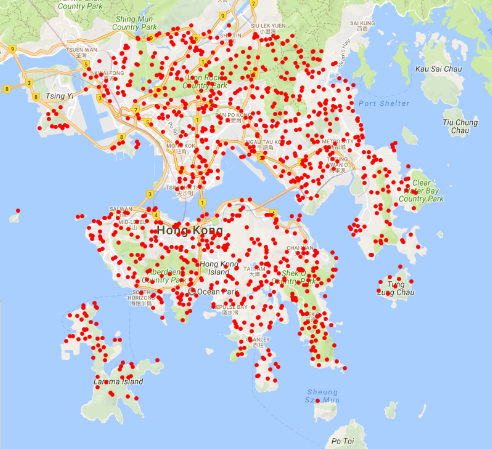
\includegraphics[scale=1]{Images/HongKong.png} 
\caption{Randomly generated locations to sample urban form in Hong Kong. <Update this figure to final methodology where 100\% blue images were removed>} 
\end{figure}


\subsection{Imagery sources}\label{sec:methods3}

For each city, three different types of imagery were used. The first is precinct-level Google Maps images were obtained at the selected locations using a custom style defined with the Google Static Maps API (see Figure \ref{fig:maps} for examples of Paris, France). The images, sized 320 by 320 pixels, provide a high-level abstraction of road (black) and public transport (orange) networks, green space (green), and water bodies (blue). Any remaining space is coded white.

The second was satellite images

The third was street view images (from google and baidu)

     
 
 
\begin{figure}[!htbp] \label{fig:maps}  
    \centering    
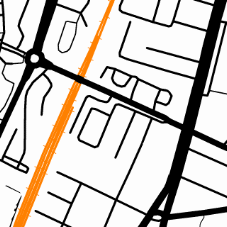
\includegraphics[scale=1]{Images/Map1.png} 
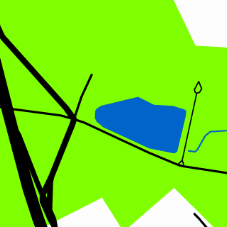
\includegraphics[scale=1]{Images/Map2.png} 
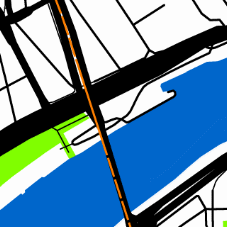
\includegraphics[scale=1]{Images/Map3.png} 
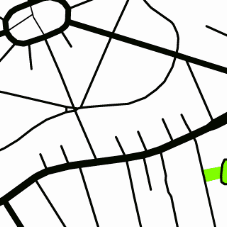
\includegraphics[scale=1]{Images/Map4.png}  
\caption{Four sample images for Paris, France (Google Maps, 2017)}    
\end{figure} 
 
 \subsection{Neural network training}\label{sec:methods4}    

To accurately calibrate the 25 million parameters of the Inception V3 architecture for any computer vision task, it is preferable to use millions of training images with high-quality labels. Therefore, 1000 samples were randomly selected from each city area, resulting in a study dataset of 1,667,000 images. This dataset, obtained using Python \citep{Python2016}, was randomly split into a training (75\%) and validation (25\%) set. In order to obtain a balanced training data set of 750 images per city, sampling was performed sequentially per city.
The Inception V3 network was calibrated using supervised learning with the generated dataset to identify the name of the city based on a supplied precinct-level image. Several pre-processing steps were performed before supplying the image to the neural network. In particular, images were randomly flipped and randomly cropped during pre-processing from 320x320x3 to Inception V3’s native 299x299x3 resolution. No zooming is applied and the aspect ratio is kept fixed, while colour transformations are not required due to our pre-specified limited colour scheme. All images were normalised to [-1, 1] by subtracting a colour value of 128 from each pixel and multiplying by 1/128. To ensure good mixing, training images were randomly allocated to batches. Validation images were transformed to 299x299x3 using central cropping.

To update weights in the neural network, a loss function has to be specified to quantify the extent of any current misclassifications. The loss function used in this study is a weighted sum of the cross entropy calculated on the softmax function output of the nodes in the final layer (77\%) and the auxiliary end nodes (23\%). Model parameters are calibrated by minimising this loss function using Stochastic Gradient Descent with Nesterov momentum of 0.9. Other parameters include a batch size of 64 samples, learning rate starting at 0.9 per batch, reduced by 6\% every two epochs, batch normalization, a dropout rate of 0.2 after the final average-pooling operations, and an L2 regularization weight per sample of 0.0001. After Glorot uniform random weight initialisation, the model was trained until convergence for a total of 200 epochs (approximately four weeks using one NVIDIA GTX 1080 GPU), using the Microsoft Cognitive Toolkit (CNTK) \citep{Yu2015}. This resulted in 86.1\% accuracy of the final model for predicting the correct city using images in the validation set (i.e., top 1 error of 13.9\%). Inference of each of the 416,750 images in the validation set also resulted in probability estimates for all 1667 classes the image could belong to. These probability estimates were used in graph-based clustering as follows.


\subsubsection{Maps}
Imagery from Google Maps was used to train CNTK. Training was run for 150 epochs with the validation step reaching an error rate of 14.625\%. 

how many cities



Imagery from Google Street View was used to train CNTK. Training was run for 150 epochs with the validation step reaching an error rate of 56.877\%.




Imagery from Google Satellite was used to train CNTK. Training was run for 150 epochs with the validation step reaching an error rate of 0.581\%.














\section{Results}\label{sec:results}

\section{Discussion}\label{sec:discussion}

\section{Conclusion}\label{sec:conclusion}


\section*{References}\label{sec:ref}
%% If you have bibdatabase file and want bibtex to generate the
%% bibitems, please use
%%
  \bibliographystyle{elsarticle-harv} 
  \bibliography{library}

%% else use the following coding to input the bibitems directly in the
%% TeX file.

\begin{thebibliography}{00}

%% \bibitem[Author(year)]{label}
%% Text of bibliographic item

\bibitem[ ()]{}

\end{thebibliography}


%% The Appendices part is started with the command \appendix;
%% appendix sections are then done as normal sections
\appendix
\setcounter{table}{0}
\renewcommand{\thetable}{A\arabic{table}}

%\subsection{}                               %% Appendix A1, A2, etc.




\end{document}

\endinput
%%
%% End of file `elsarticle-template-harv.tex'.
